\documentclass[aspectratio=169]{beamer}
\setbeamertemplate{navigation symbols}{}
\usepackage{color,amsmath,comment, subfigure}
\usepackage{booktabs}
\usepackage{url}

%%%%%%%%%%%%%%%%%%%%%%%%%%
\title[]{The connected age and the small world problem}
\author[]{Matthew J. Salganik}
\institute[]{Social Networks (Soc 204)\\Princeton University}
\date[]{Wednesday, September 8, 2021\\Week 2, Lecture 2\\ 
\vfill

\begin{flushleft}
\vspace{0.7in}

\includegraphics[width=0.05\textwidth]{figures/cc.png}
\end{flushleft}
}

\note{
equipment you will need:
folder and coin for attrition demo
}

\begin{document}
%%%%%%%%%%%%%%%%%%%%%%%%%%%
\frame{\titlepage}
%%%%%%%%%%%%%%%%%%%%%%%%%%%
\begin{frame}

Expectations about reading and lecture:
\begin{itemize}
\item I expect you to watch the pre-read video
\pause
\item I expect you to read the materials
\pause
\item In the lecture, I will do a mix of reviewing the reading, providing context, and discussing extensions 
\end{itemize}

\end{frame}
%%%%%%%%%%%%%%%%%%%%%%%%%%%
\begin{frame}

\begin{enumerate}
\item Watts, Preface and Chapter 1.
\item Milgram, S. (1967). The small world problem. \textit{Psychology Today}.
\item Travers, J. and Milgram, S. (1969). An experimental study of the small world problem. \textit{Sociometry}.
\item Kleinfeld, J.S. (2002). The small world problem. \textit{Society}.
\end{enumerate}

\end{frame}
%%%%%%%%%%%%%%%%%%%%%%%%%%%
\begin{frame}

\begin{columns}
\begin{column}{0.5\textwidth}
  \begin{center}
    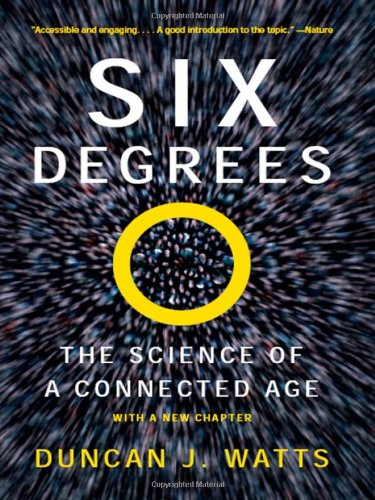
\includegraphics[width=0.50\textwidth]{figures/watts_six_2003_cover}
  \end{center}
\end{column}
\begin{column}{0.5\textwidth}  
\pause
    \begin{center}
     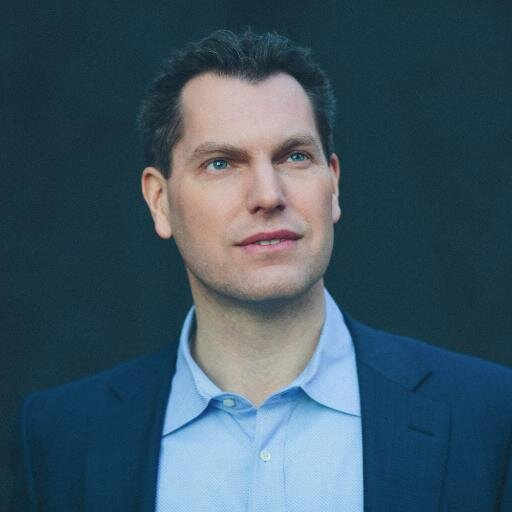
\includegraphics[width=0.5\textwidth]{figures/duncan_headshot}
     \end{center}
\end{column}
\end{columns}

\note{
This book has an author.  He is just a normal person.  I love this book because it shows science in action.  So, when stuff from our precept turns out messy or unexpected that's normal.  This book shows what science is really like: being stuck and confused a lot.
}

\end{frame}
%%%%%%%%%%%%%%%%%%%%%%%%%%%
\begin{frame}

\begin{center}
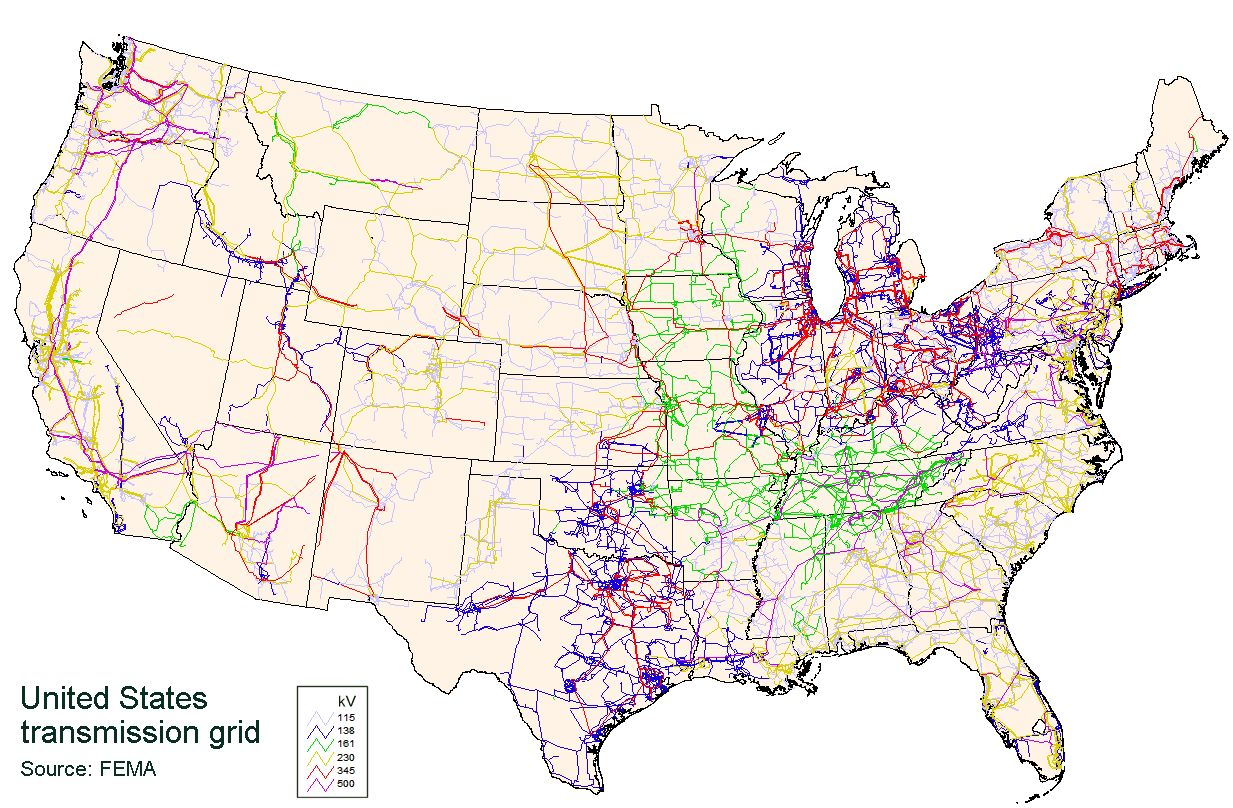
\includegraphics[width=0.8\textwidth]{figures/power_grid}
\end{center}

\vfill
\tiny{\url{https://commons.wikimedia.org/wiki/File:UnitedStatesPowerGrid.jpg}}

\note{
cascading failure in power grid.  Single line failing in Oregon puts strain on other lines and systems.  This causes more failure, which means more strain which means more failure.
cascading failure in the financial system.  Government bails out AIG 85 billion dollars.  They do it because they are worried about this in the financial system.
}

\end{frame}
%%%%%%%%%%%%%%%%%%%%%%%%%%%
\begin{frame}

\begin{center}
\Large{
How does individual behavior aggregate\\ to collective behavior?
}
\end{center}

\note{
Sociology is about: Dog and pack of dogs
Jury members of Juries
Crickets and packs of crickets (how are these crickets connected together)?
}

\end{frame}
%%%%%%%%%%%%%%%%%%%%%%%%%%%%
\begin{frame}

The small world problem

\end{frame}
%%%%%%%%%%%%%%%%%%%%%%%%%%%%%
\begin{frame}

\begin{center}
\Large{
``Oh my goodness.  It's a small world!''
}
\end{center}

When was the last time you said this?  Think-pair-share

\end{frame}
%%%%%%%%%%%%%%%%%%%%%%%%%%%
\begin{frame}

\begin{center}
\Large{
``Oh my goodness.  It's a small world!''
}
\end{center}

\pause
Two times that people say this:
\begin{itemize}
\item See someone they know in an unexpected place
\pause
\item Meet someone and find out that they have an acquaintance in common
\end{itemize}

\note{
When was the last time you said this?  Think-pair-share.  
Two kinds of experiences. You see someone you know at an unexpected place.  You figure out that you have a friend in common 
}

\end{frame}
%%%%%%%%%%%%%%%%%%%%%%%%%%%
\begin{frame}

Let's think back to 1967 . . . . 

\end{frame}
%%%%%%%%%%%%%%%%%%%%%%%%%%%
\begin{frame}

\begin{center}
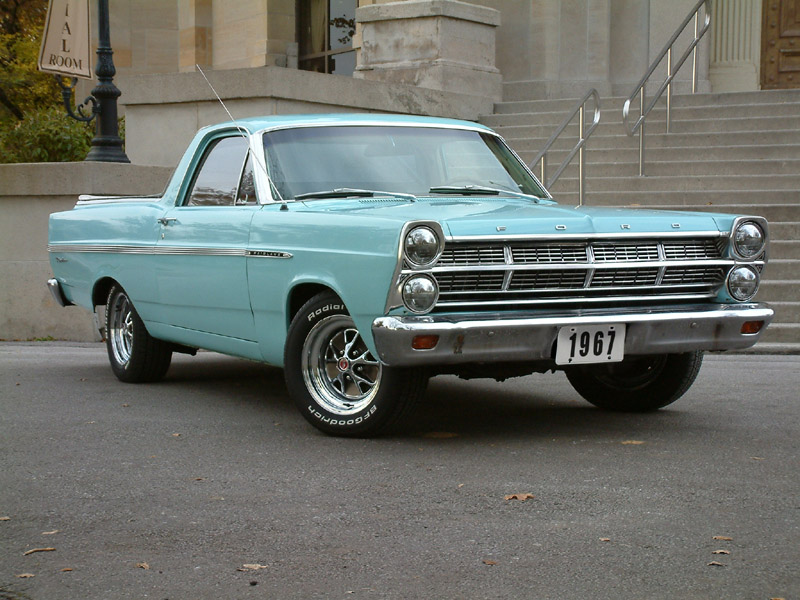
\includegraphics[height=0.8\textheight]{figures/1967_Ford_Fairlane_Ranchero.jpg}
\end{center}

\vfill
\tiny{\url{http://upload.wikimedia.org/wikipedia/commons/f/f5/1967_Ford_Fairlane_Ranchero.jpg}}

\end{frame}
%%%%%%%%%%%%%%%%%%%%%%%%%%%
\begin{frame}

\begin{center}
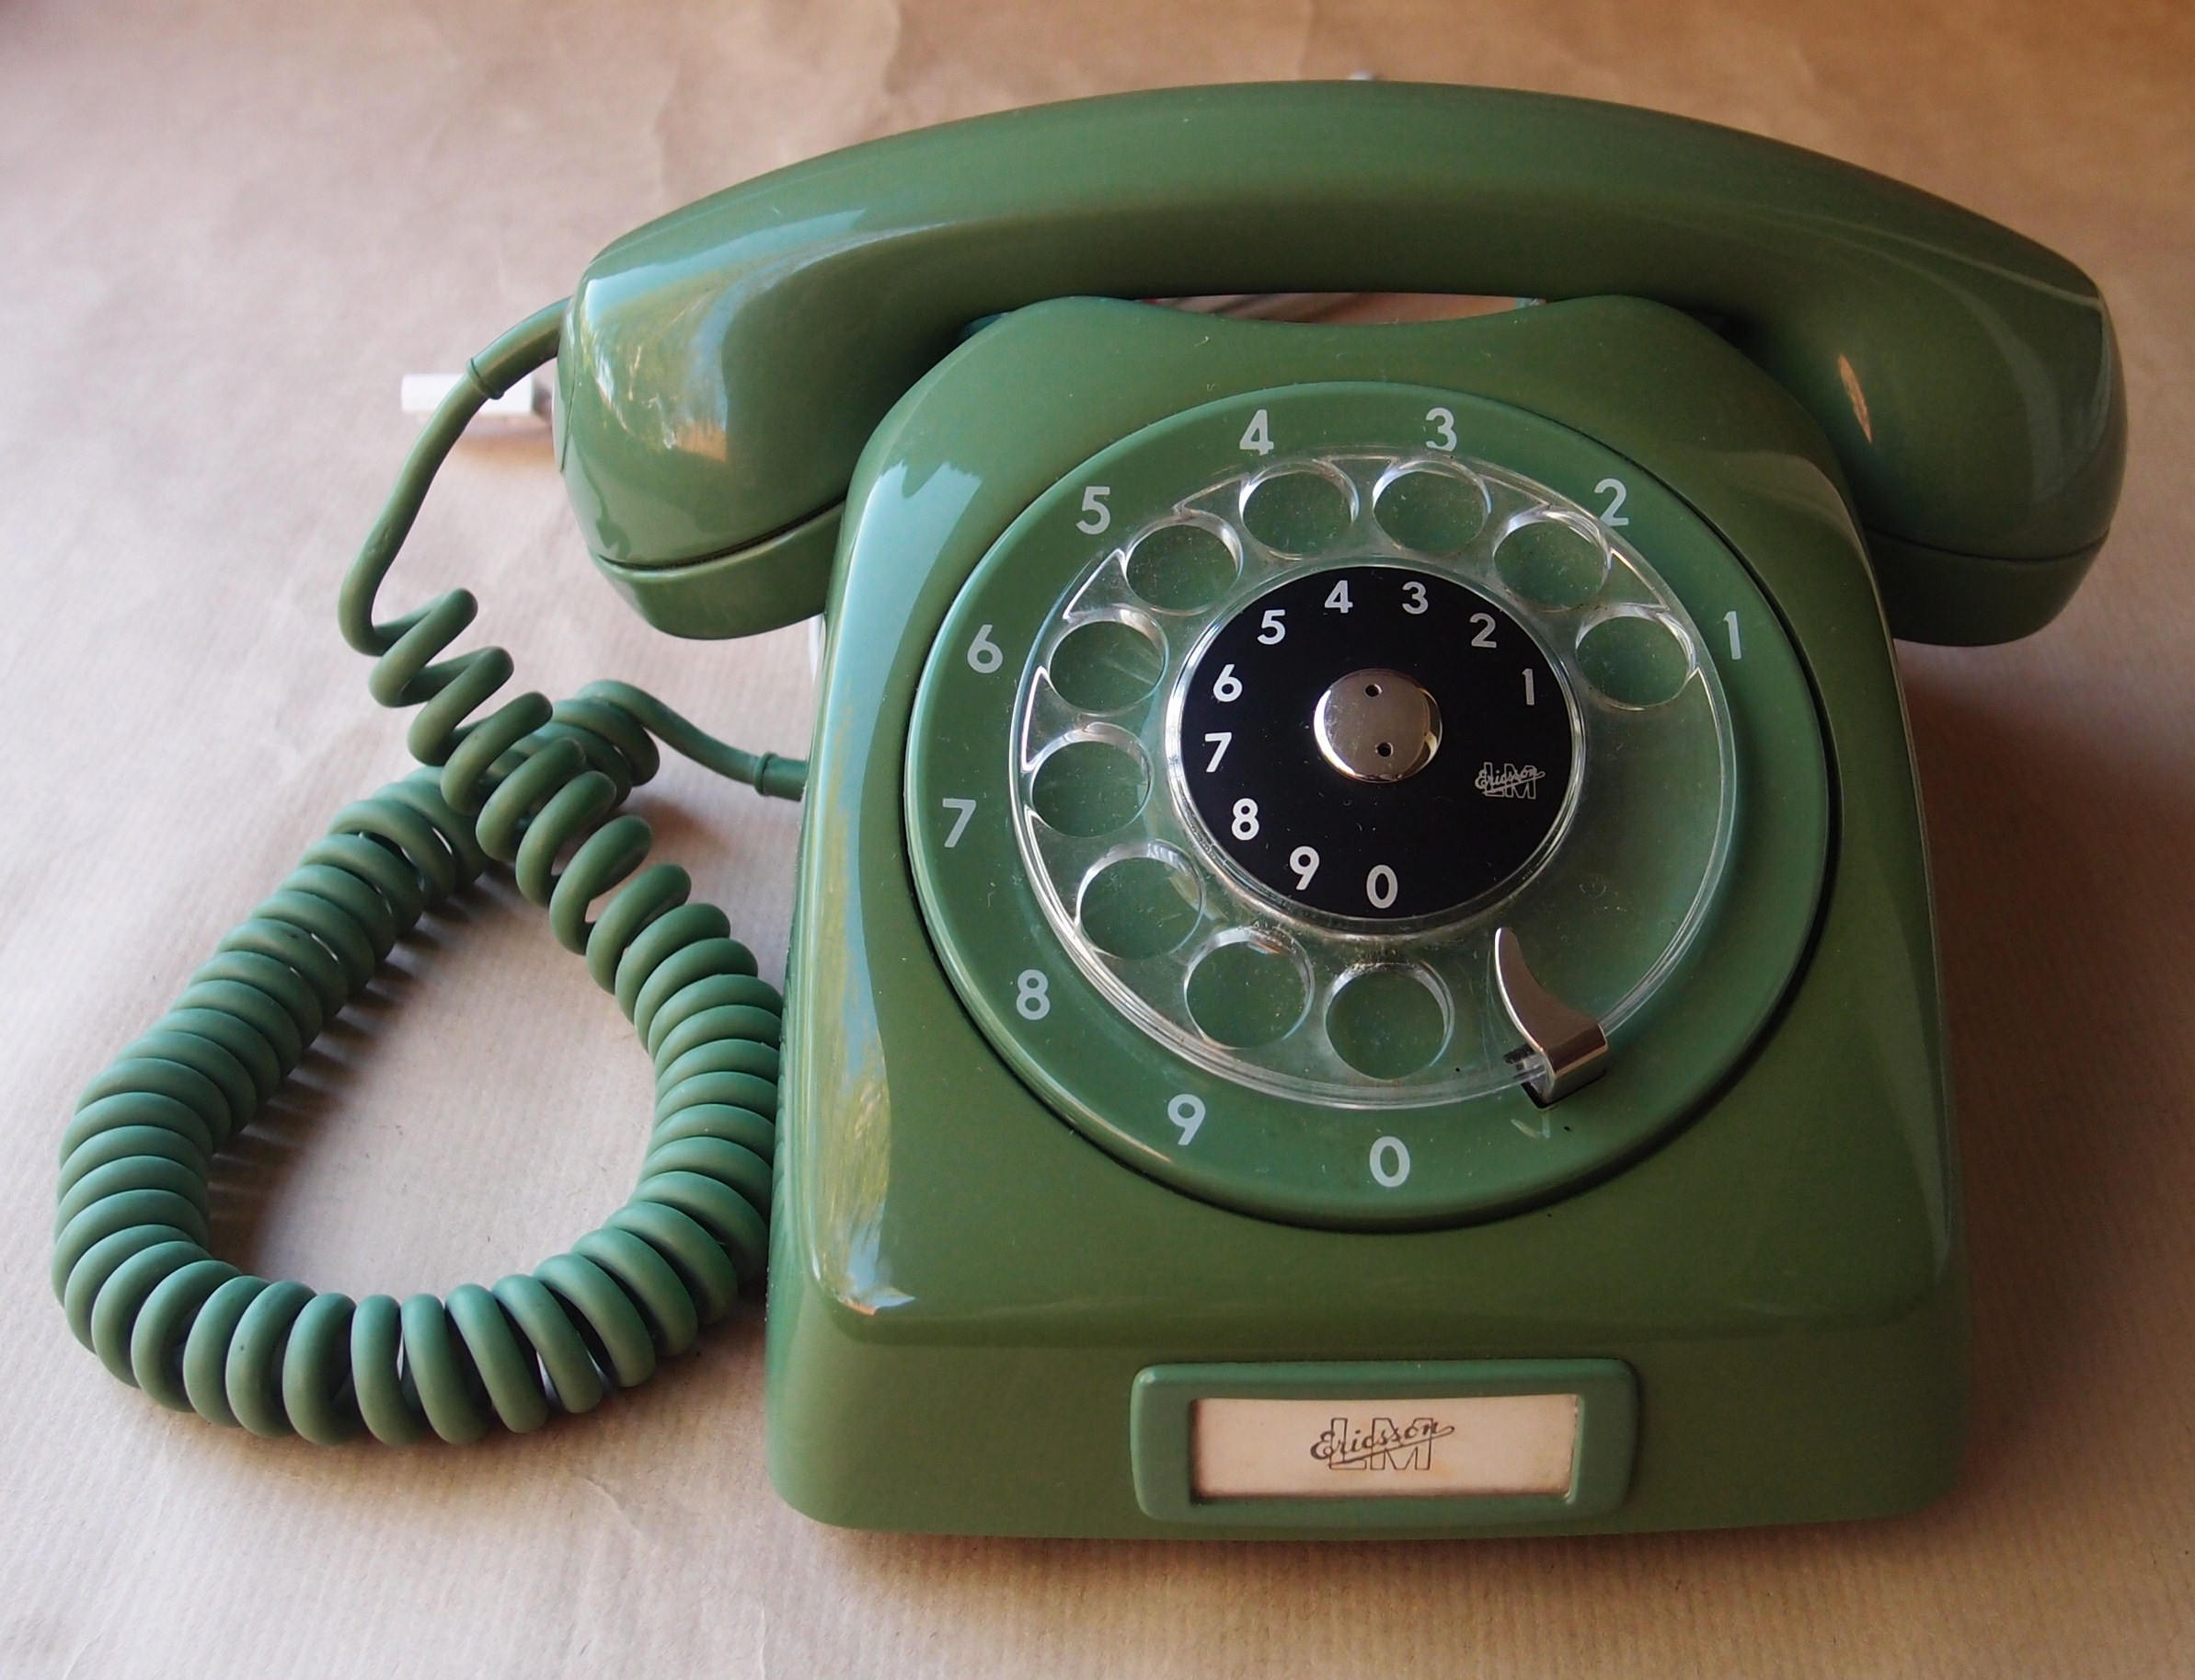
\includegraphics[height=0.8\textheight]{figures/Ericsson_Dialog_in_green}
\end{center}

\vfill
\tiny{\url{http://commons.wikimedia.org/wiki/File:Ericsson_Dialog_in_green.JPG}}

\end{frame}
%%%%%%%%%%%%%%%%%%%%%%%%%%%
\begin{frame}

\begin{center}
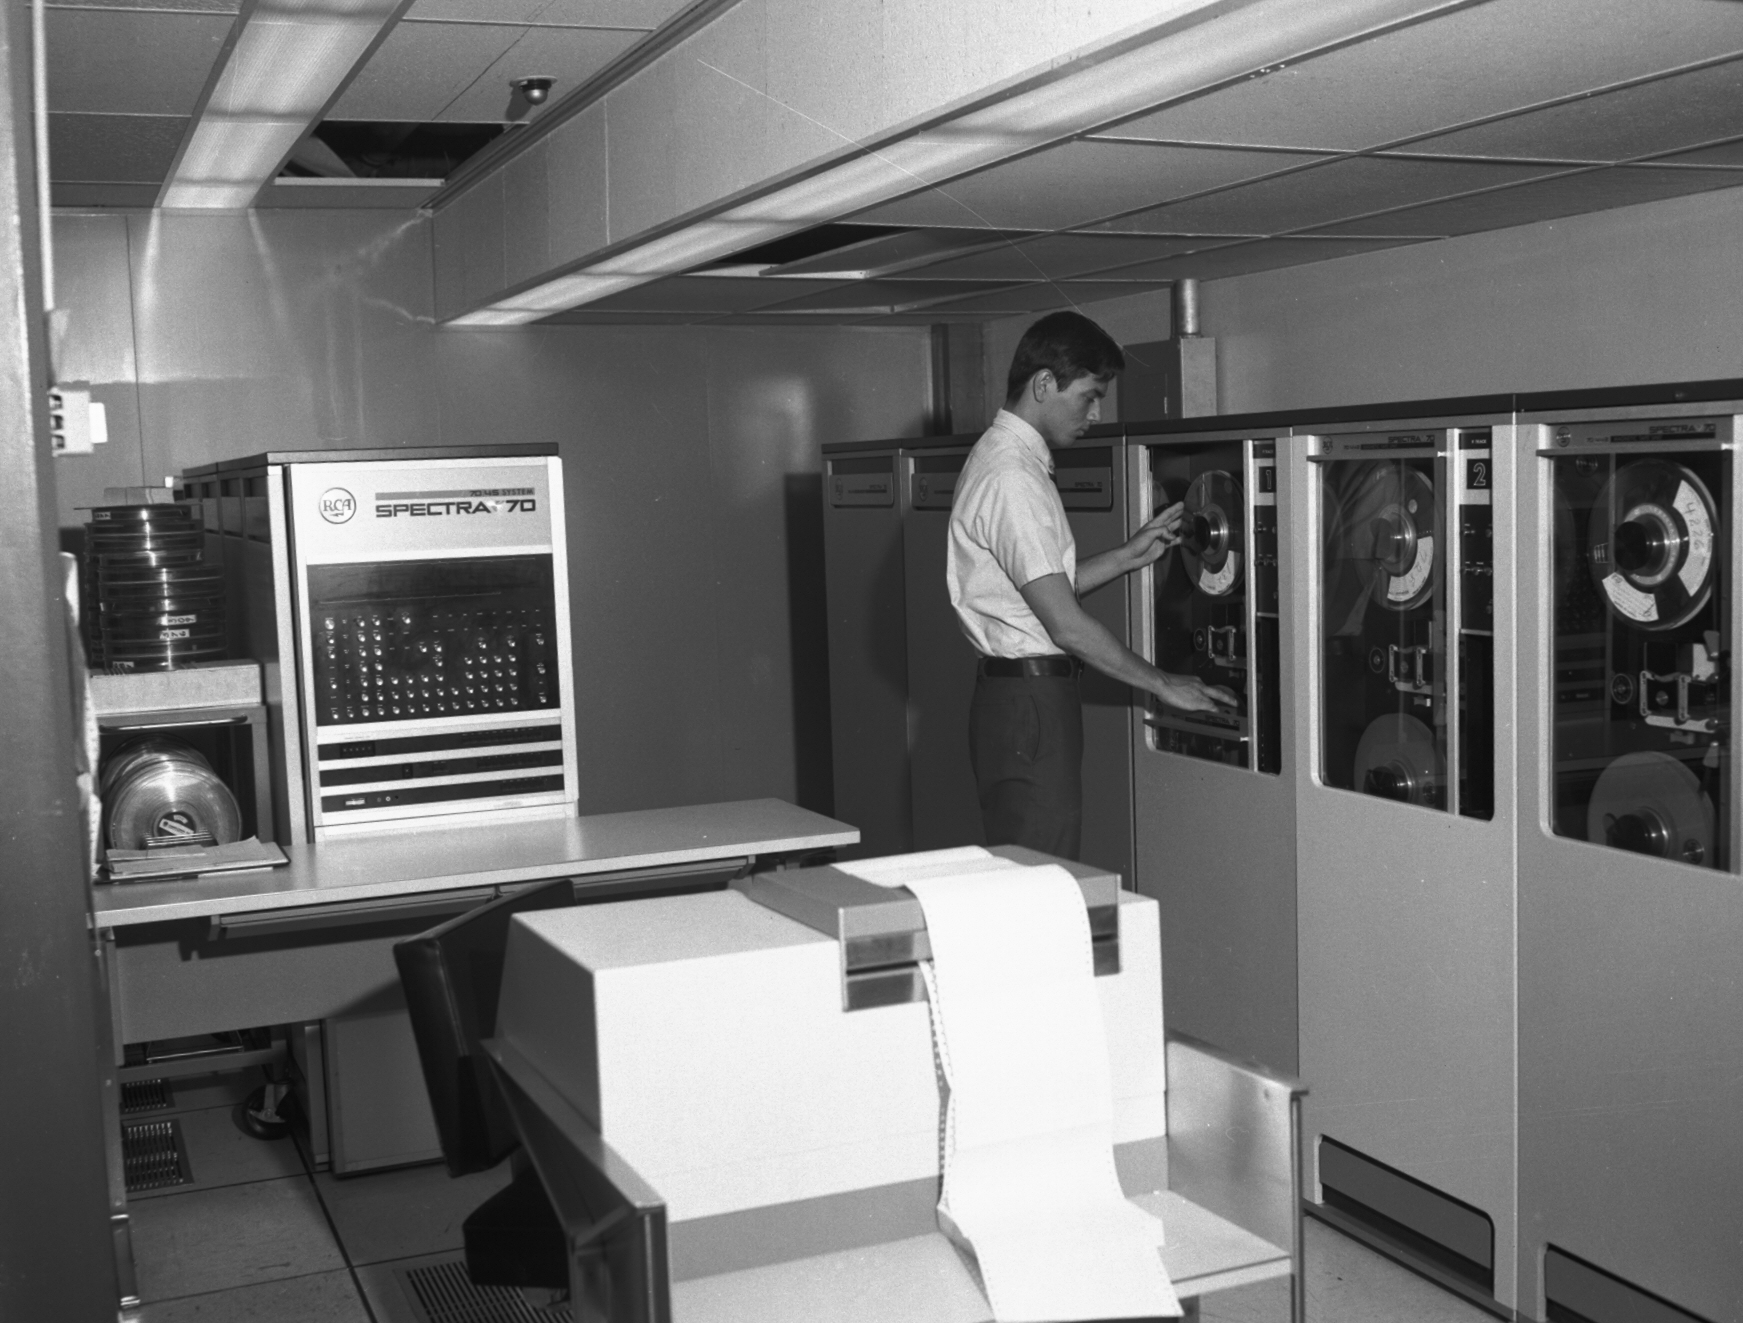
\includegraphics[height=0.8\textheight]{figures/Computer_in_County_of_Orange_offices,_1967}
\end{center}

\vfill
\tiny{\url{http://commons.wikimedia.org/wiki/File:Computer_in_County_of_Orange_offices,_1967.jpg}}

\end{frame}
%%%%%%%%%%%%%%%%%%%%%%%%%%%
\begin{frame}

Fred Jones of Peoria, sitting in a sidewalk cafe in Tunis, and needing a light for his cigarette, asks the man at the next table for a match. They fall into conversation; the stranger is an Englishman who, it turns out, spent several months in Detroit studying the operation of an interchangeable-bottlecap-factory. ``I know it's a foolish question'' says Jones, ``but did you ever by any chance run into a fella named Ben Arkadian? He's an old friend of mine, manages a chain of supermarkets in Detroit . . . '' ``Arkadian, Arkadian'' the Englishman mutters. ``Why, upon my soul, I believe I do! Small chap, very energetic, raised merry hell with the factory over a shipment of defective bottlecaps.'' ``No kidding!'' Jones exclaims in amazement. ``Good lord, it's a small world isn't it!''

\vfill
Milgram (1967)
\end{frame}
%%%%%%%%%%%%%%%%%%%%%%%%%%%
\begin{frame}

\begin{itemize}
\item What is the probability that two people chosen at random know each other?
\pause
\item What is the probability that two people chosen at random share a friend?
\pause
\item Given two individuals selected randomly from the population, what is the probability that the minimum number of intermediaries required to link them is 0,1,2,...k?
\end{itemize}

\end{frame}
%%%%%%%%%%%%%%%%%%%%%%%%%
\begin{frame}

\begin{center}
Modeling approach (i.e., MIT approach)\\
  vs.\\
Empirical approach (i.e., Harvard approach)
\end{center}

\note{
We will see more of the modeling approach next week
}

\end{frame}
%%%%%%%%%%%%%%%%%%%%%%%%%
\begin{frame}

\begin{center}
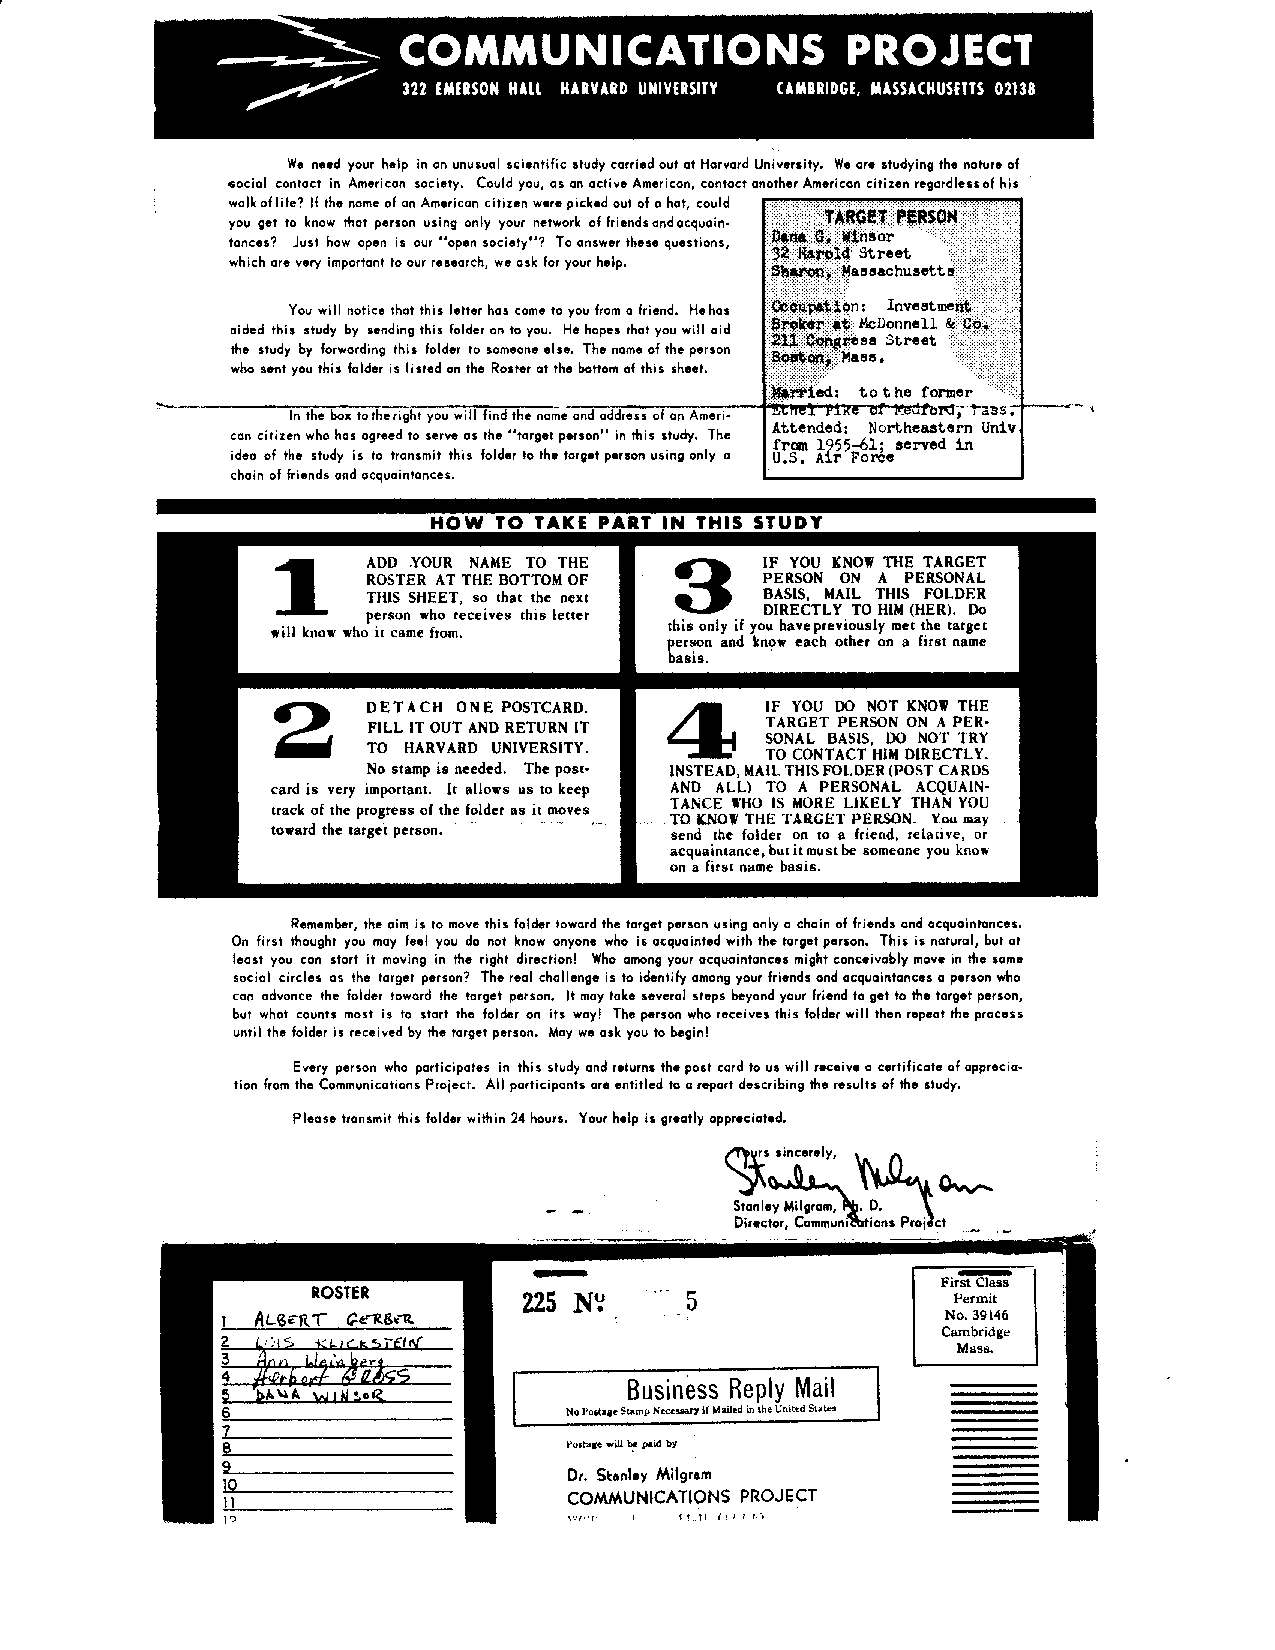
\includegraphics[height=0.9\textheight]{figures/small_world_dossier}
\end{center}

\end{frame}
%%%%%%%%%%%%%%%%%%%%%%%%
\begin{frame}

This procedure is elegant.\pause

\begin{itemize}
\item provides a view of the big invisible social network of Americans
\pause
\item flexible in choice of starters and targets
\pause
\item tracer cards provide data on incomplete chains (and demographics of participants)
\end{itemize}

\note{
flexible in choice of starters
and choice of targets
tracer cards provide data on incomplete chains (and demographics of participants)
also flexible in the type of information provided about the target

There is a big invisible web, and this gives us tracers through it
}

\end{frame}
%%%%%%%%%%%%%%%%%%%%%%%%
\begin{frame}

Results

\end{frame}
%%%%%%%%%%%%%%%%%%%%%%%%%
\begin{frame}
\frametitle{Result 1}

\begin{center}
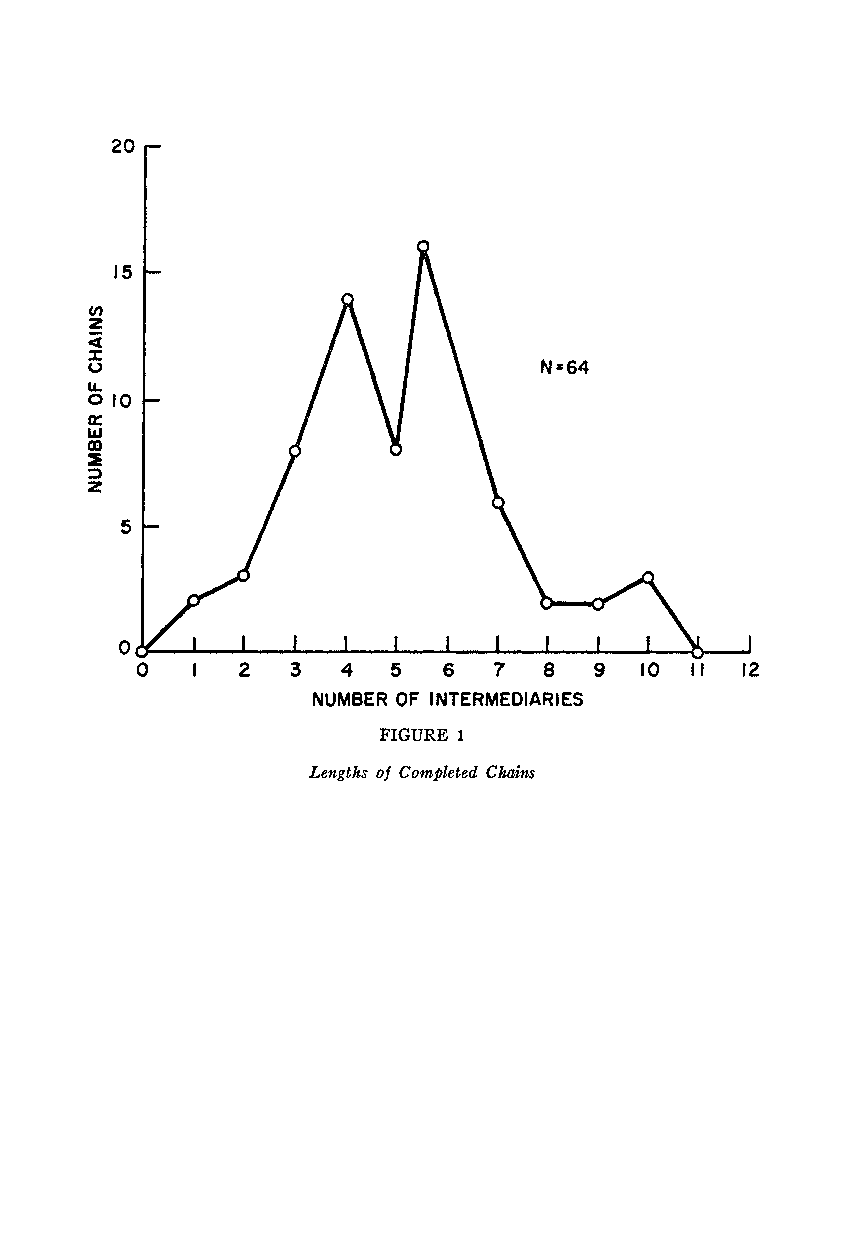
\includegraphics[height=0.7\textheight]{figures/travers_experimental_1969_fig1}
\end{center}

Mean number of intermediaries: 5.2\\ 

\end{frame}
%%%%%%%%%%%%%%%%%%%%%%%%%%%
\begin{frame}
\frametitle{Result 1}

\begin{itemize}
\item 1 intermediary = 2 ``degrees of separation''
\pause
\item 5 intermediaries = 6 ``degrees of separation''
\end{itemize}

\end{frame}
%%%%%%%%%%%%%%%%%%%%%%%%%%%
\begin{frame}
\frametitle{Result 2}

\begin{itemize}
\item Travers and Milgram: 29\% of chains reached target
\pause
\item Kleinfeld: 71\% of chains did not reach target
\end{itemize}

\pause
Be careful as you read.

\note{
scientists call attention to make their work look good (similar to politicians)
folder demo
more likely to see short chains than long chains
}

\end{frame}
%%%%%%%%%%%%%%%%%%%%%%%%%%%
\begin{frame}

\begin{itemize}
\item How should we interpret the distribution of chain lengths in the presence of chains that don't complete?
\pause
\item Demo of the effects of random attrition
\pause
\item Chains that complete will tend to be shorter than chains that don't complete (you will see this again in reading for next class).
\pause
\item General lesson: Think about the data you see and the data you don't see.  If the data you don't see are systematically different from the data you see, be careful.
\end{itemize}

\end{frame}
%%%%%%%%%%%%%%%%%%%%%%%%%%%
\begin{frame}
\frametitle{Result 3}

\begin{center}
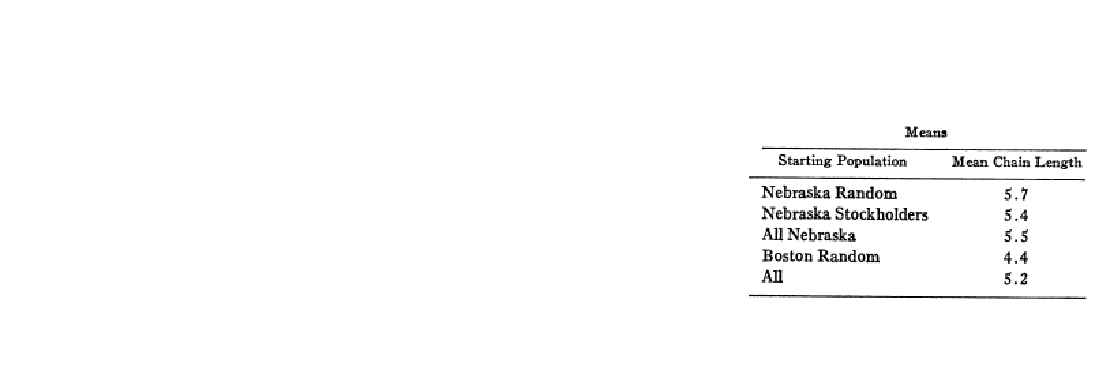
\includegraphics[height=0.6\textheight]{figures/travers_experimental_1969_tab2b}
\end{center}
\pause
\vfill
What does this design reveal about Travers and Milgram?
\note{
Anyone here from Nebraska
What does this design reveal about Milgram?
This is also why it is important to have people from many backgrounds and experiences doing research.  Who you are and what you have experienced impacts the questions you ask.
}

\end{frame}
%%%%%%%%%%%%%%%%%%%%%%%%%%%
\begin{frame}
\frametitle{Result 4}

\begin{center}
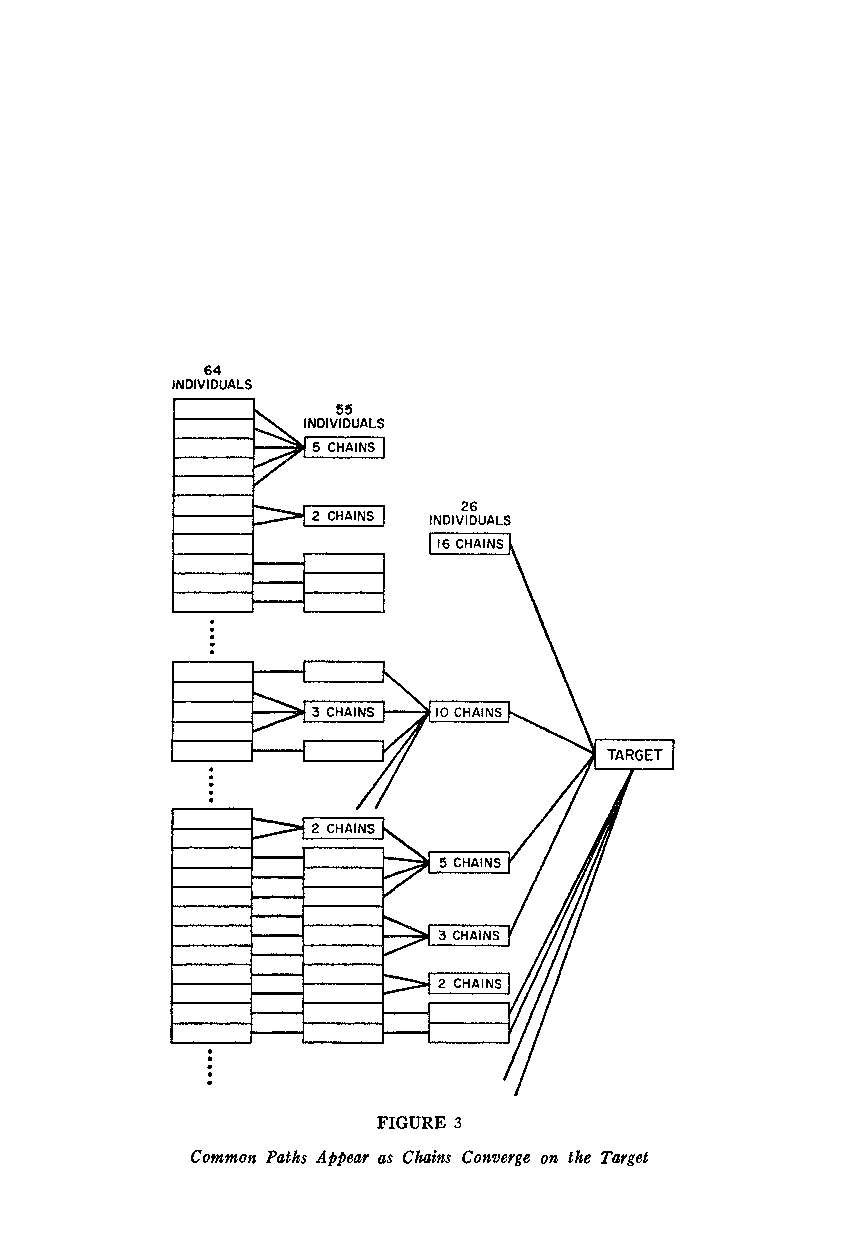
\includegraphics[height=0.9\textheight]{figures/travers_experimental_1969_fig3}
\end{center}


\end{frame}
%%%%%%%%%%%%%%%%%%%%%%%%%
\begin{frame}
\frametitle{Result 4}

\begin{center}
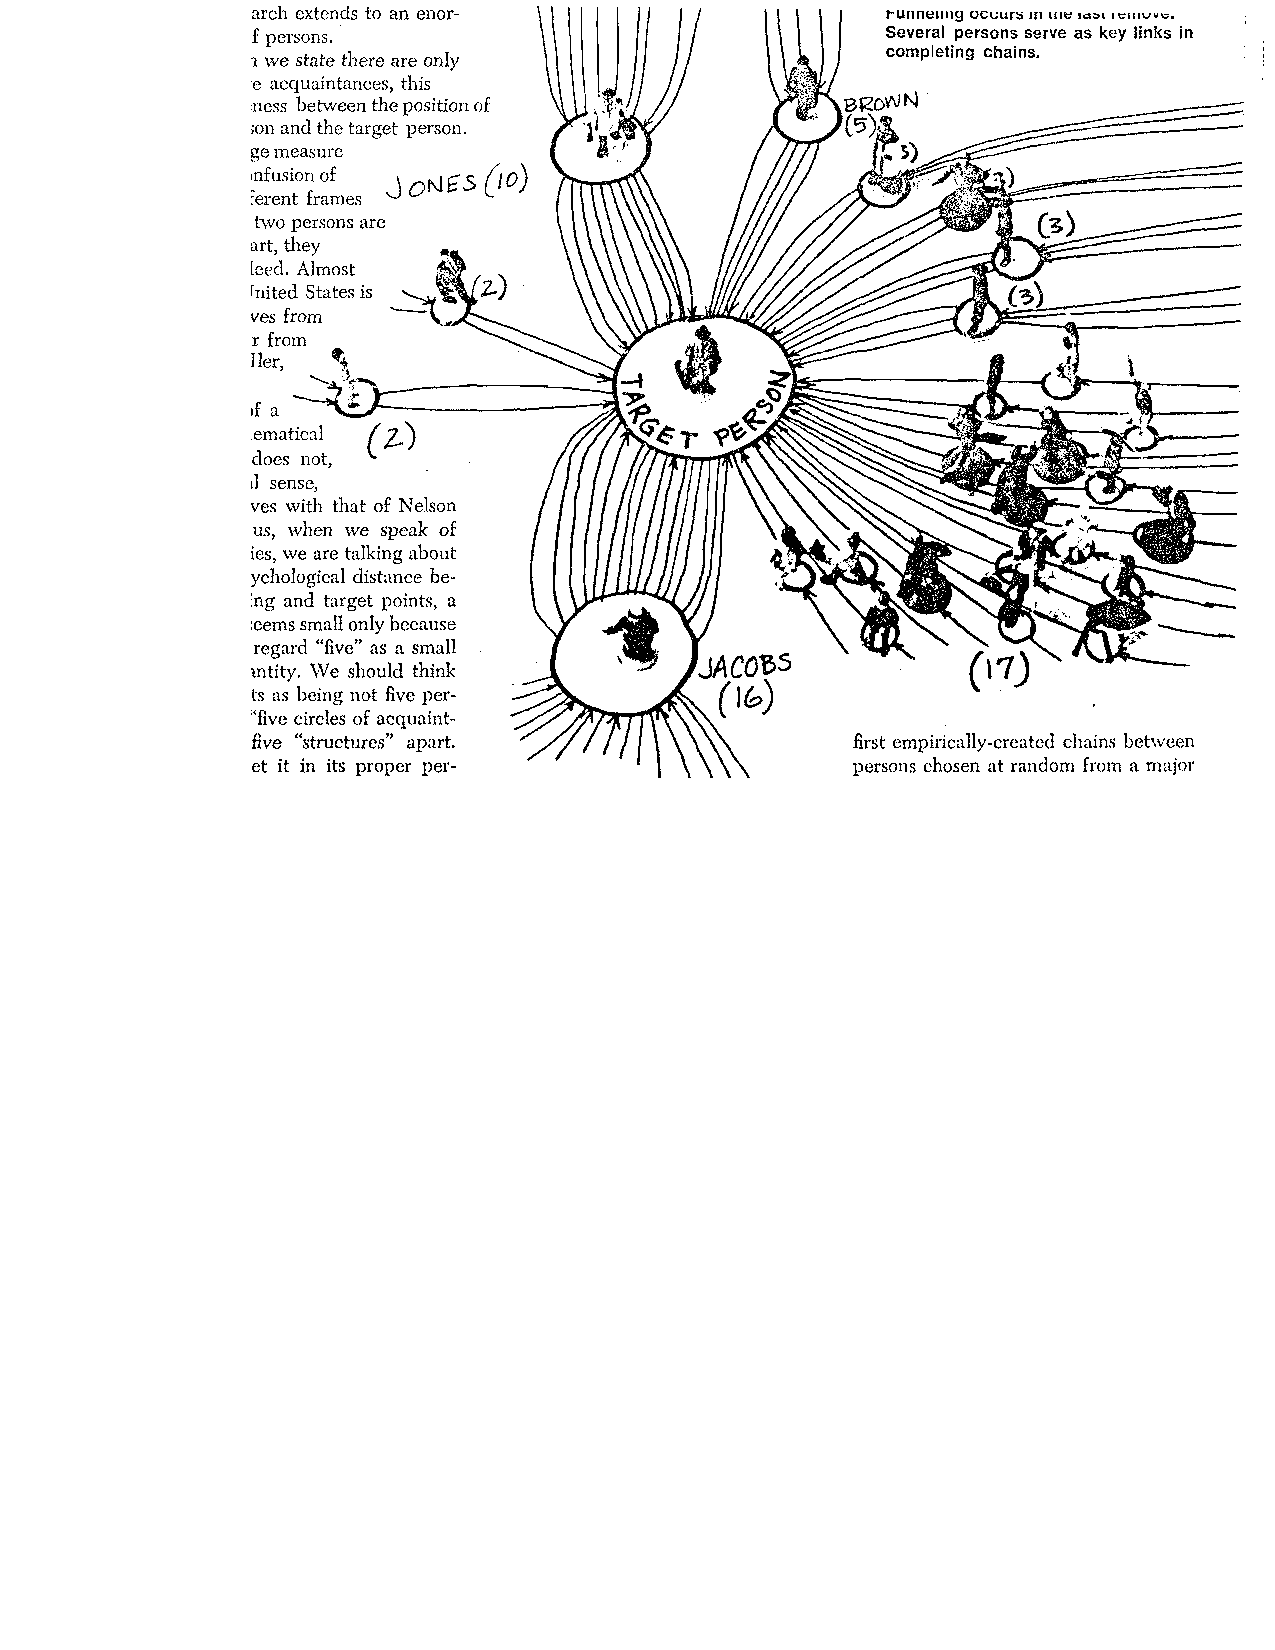
\includegraphics[height=0.8\textheight]{figures/milgram_small-world_1967_funneling}
\end{center}

Funneling, will be the subject of future work

\end{frame}
%%%%%%%%%%%%%%%%%%%%%%%%%
\begin{frame}
\frametitle{}

This is just one of many possible small world experiments. Milgram choose to do others. Let's see what he did. . .

\end{frame}
%%%%%%%%%%%%%%%%%%%%%%%%%
\begin{frame}

\begin{center}
\includegraphics<1>[height=0.8\textheight]{figures/1967_Ford_Fairlane_Ranchero.jpg}
\end{center}

\vfill
\tiny{\url{http://upload.wikimedia.org/wikipedia/commons/f/f5/1967_Ford_Fairlane_Ranchero.jpg}}

\end{frame}
%%%%%%%%%%%%%%%%%%%%%%%%%%%
\begin{frame}

\begin{center}
\includegraphics<1>[height=0.8\textheight]{figures/Ericsson_Dialog_in_green}
\end{center}

\vfill
\tiny{\url{http://commons.wikimedia.org/wiki/File:Ericsson_Dialog_in_green.JPG}}

\end{frame}
%%%%%%%%%%%%%%%%%%%%%%%%%%%
\begin{frame}

\begin{center}
\includegraphics<1>[height=0.8\textheight]{figures/Computer_in_County_of_Orange_offices,_1967}
\end{center}

\vfill
\tiny{\url{http://commons.wikimedia.org/wiki/File:Computer_in_County_of_Orange_offices,_1967.jpg}}

\end{frame}
%%%%%%%%%%%%%%%%%%%%%%%%%%%
\begin{frame}

\begin{center}
\includegraphics<1>[height=0.8\textheight]{figures/detriot_race_riot_1967}
\end{center}

\vfill
\tiny{\url{http://content.time.com/time/covers/0,16641,19670804,00.html}}\\
Detroit 12th street riots: more than 40 people died, more than 1,000 injured, and more than 2,000 buildings destroyed

\end{frame}
%%%%%%%%%%%%%%%%%%%%%%%%%%%
\begin{frame}

\begin{center}
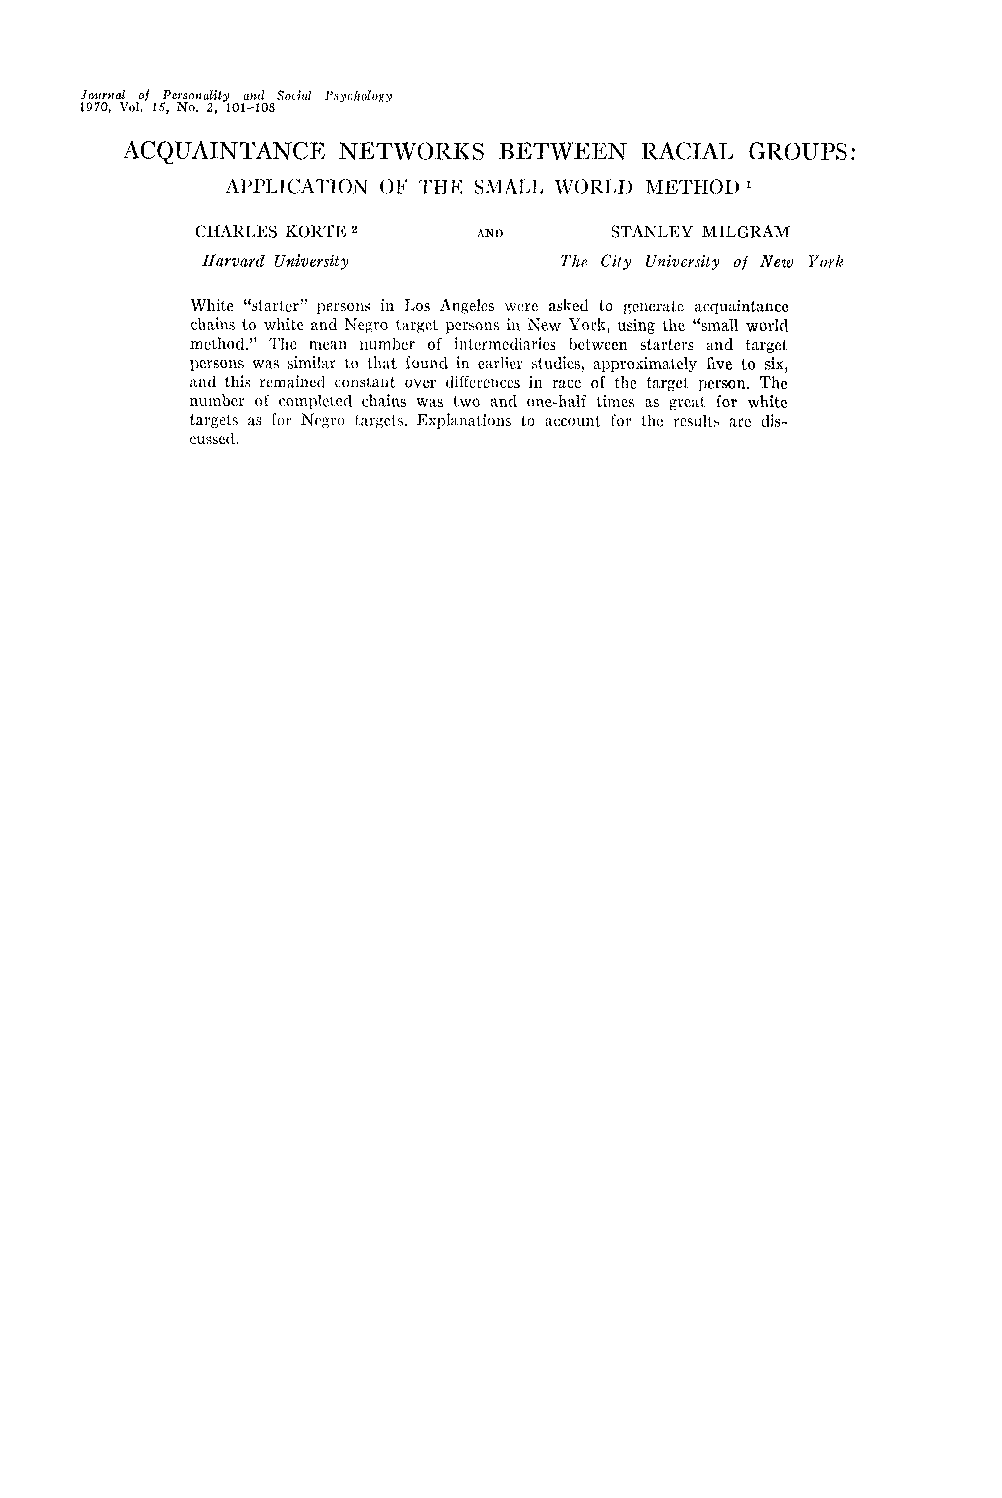
\includegraphics[width=0.9\textwidth]{figures/korte_aquaintance_1970_title}
\end{center}

\vfill
\url{http://dx.doi.org/10.1037/h0029198}

\end{frame}
%%%%%%%%%%%%%%%%%%%%%%%%%
\begin{frame}

540 white starters in LA\\
\pause

18 targets:
\begin{center}
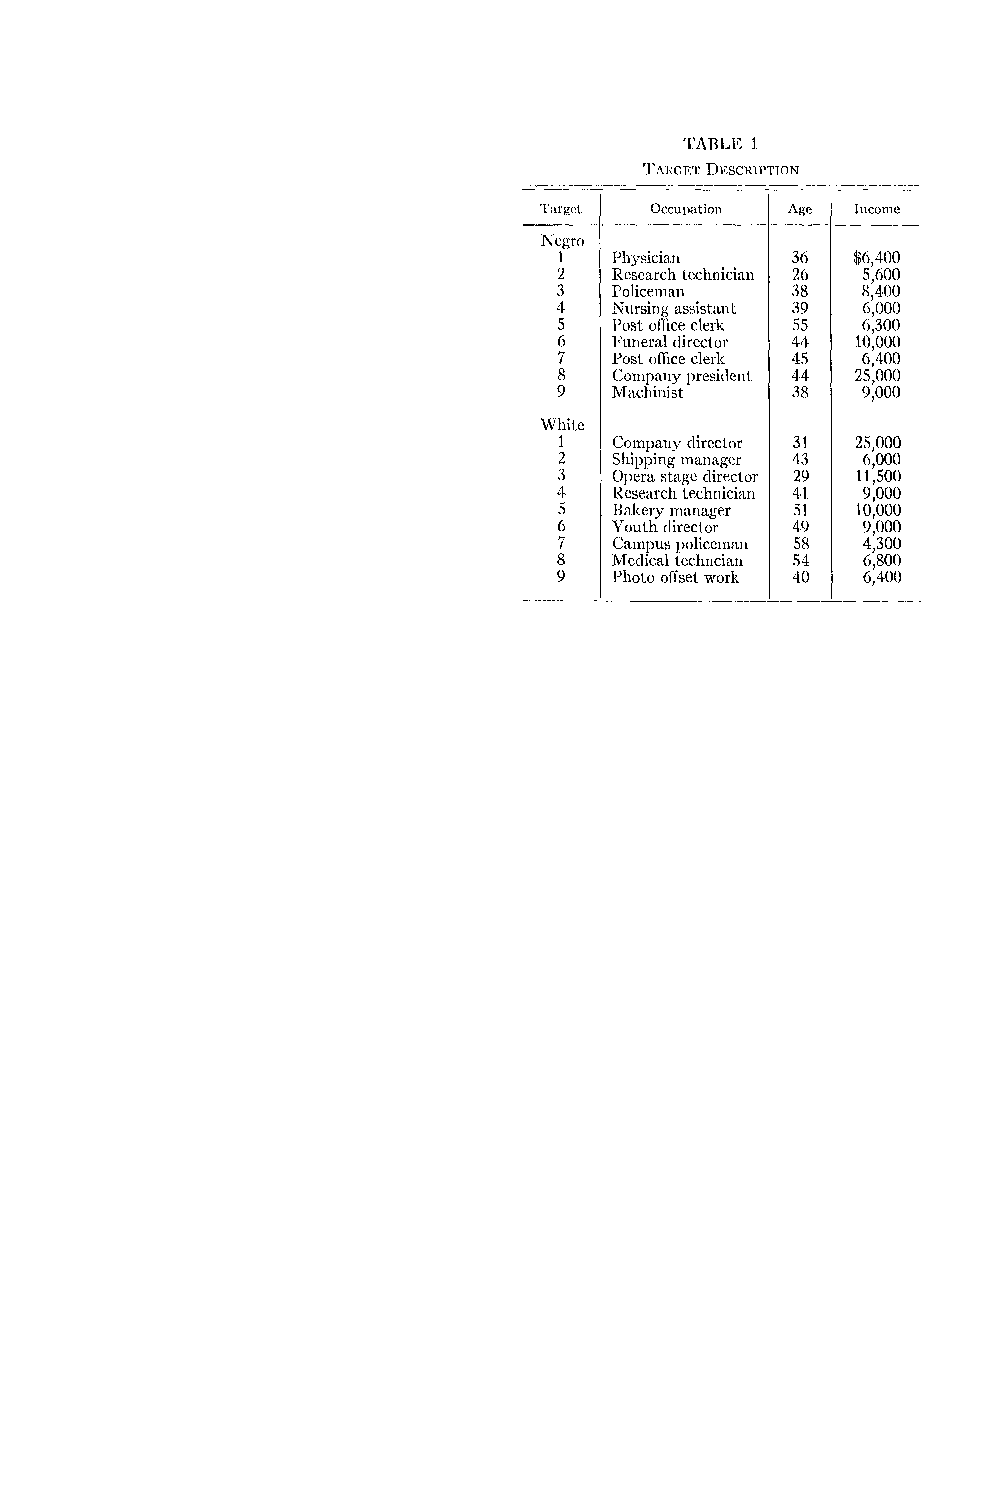
\includegraphics[height=0.6\textheight]{figures/korte_aquaintance_1970_tab1}
\end{center}

\vfill
Race of target was not explicitly known to participants

\note{
Note how Milgram spends his complexity, doesn't vary starter location any more, chooses to vary something else
}

\end{frame}
%%%%%%%%%%%%%%%%%%%%%%%%%
\begin{frame}
\frametitle{Result 1}

\begin{center}
\includegraphics<1>[height=0.8\textheight]{figures/korte_aquaintance_1970_fig1}
\end{center}

Mean intermediaries: 5.5 (white targets), 5.9 (Black targets)

\end{frame}
%%%%%%%%%%%%%%%%%%%%%%%%
\begin{frame}
\frametitle{Result 2}

\begin{center}
\includegraphics<1>[width=0.8\textwidth]{figures/korte_aquaintance_1970_tab2}
\end{center}

\vfill
Completion rate: about 30\% (white targets), about 10\% (Black targets)

\note{
What was the incompletion rate?
}

\end{frame}
%%%%%%%%%%%%%%%%%%%%%%%%
\begin{frame}
\frametitle{Result 3: Gate keepers}

\begin{center}
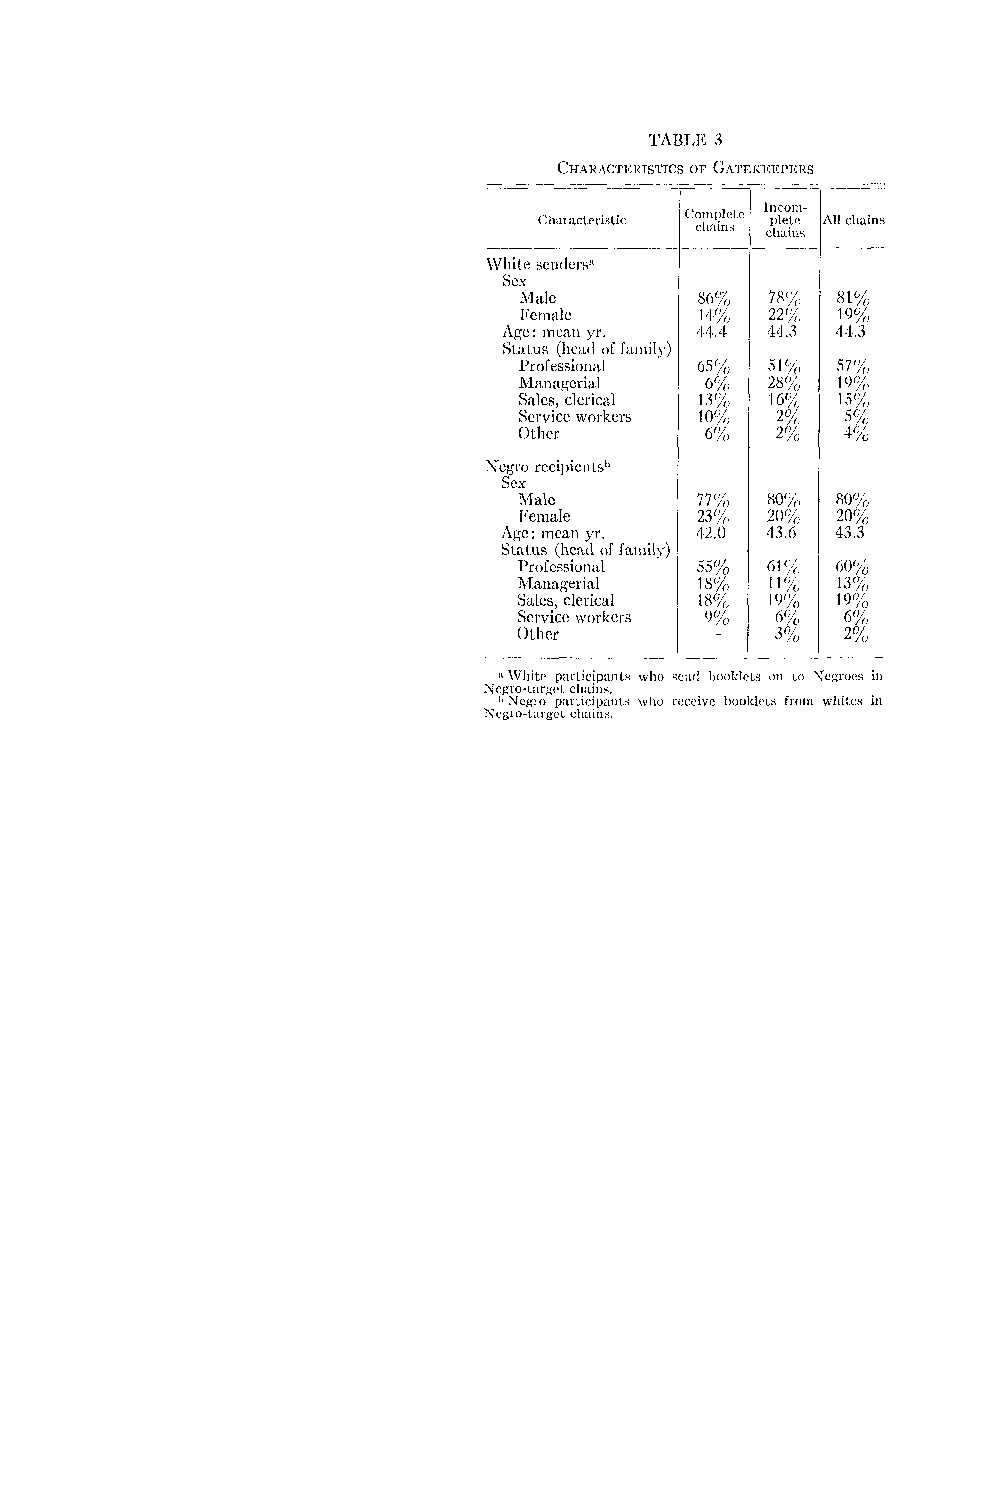
\includegraphics[height=0.6\textheight]{figures/korte_aquaintance_1970_tab3}
\end{center}

\vfill
``Gatekeepers'' of white to Black connections were predominately Male professionals\\
In 23 of the 35 successful cross-group chains, the first Black person was the target\\
Most failed chains (80\%) never crossed the racial boundary\\

\end{frame}
%%%%%%%%%%%%%%%%%%%%%%%%
\begin{frame}

\begin{itemize}
\item Introduction to the connected age
\pause
\item Small world problem shows the scientific arc: idea $\rightarrow$ formal question $\rightarrow$ empirical research $\rightarrow$ critique
\end{itemize}

\end{frame}
%%%%%%%%%%%%%%%%%%%%%%%%%
\begin{frame}

Next class: More on the small world problem and some history

\end{frame}
%%%%%%%%%%%%%%%%%%%%%%%%%
\begin{frame}

\Large{\url{http://bit.ly/soc204-2021}}

\end{frame}
%%%%%%%%%%%%%%%%%%%%%%%%%




\end{document}
